% !TEX root = thesis.tex

\section{Propietats sobre nusos}\label{sec:Propietats_sobre_nusos}

En aquesta Secció posarem de manifest diferents propietats d'un nus que més endavant tindran importància en la seva classificació.

\begin{definition}\label{def:ordre}
	Anomenem \underline{ordre} de $K$, $O(K)$ al mínim nombre de creuament que aquest pot arribar a presentar donat un diagrama qualsevol.
\end{definition}

La Figura \ref{fig:culpritknot} demostra que l'ordre del nus Culprit és zero ja que aquest sempre és un nombre positiu. Tampoc és molt difícil veure que donat un nus $K$ qualsevol a aquest se li pot afegir creuaments mitjançant moviments RI, no obstant $O(K)$ es manté contant.

\begin{definition}\label{def:nusemmirallat}
	Diem que un nus és l'\underline{emmirallat} $\overline{K}$ d'un altre nus $K$ si aquest primer s'obté a partir de l'original canviant tots els creuaments de sobrepassos a sotapassos i a la inversa.
\end{definition}

La Figura \ref{fig:nus emmirallat} mostra un exemple d'un nus emmirallat.\\

\begin{figure}
	\resizebox{6.5cm}{!}{
		\begin{tikzpicture}[line width=0.5mm, use Hobby shortcut]
			\begin{scope}
				\begin{knot}[
					consider self intersections=true,
					%  draft mode=crossings,
					ignore endpoint intersections=false,
					flip crossing/.list={1,5,6},
					only when rendering/.style={
						%    show curve endpoints
					}
					]
					\strand ([closed]0,0) .. (1.5,1) .. (.5,2) .. (-.5,1) .. (.5,0) .. (0,-.5) .. (-.5,0) .. (.5,1) .. (-.5,2) .. (-1.5,1) .. (0,0);
				\end{knot}
				\path (0,-.7);
			\end{scope}
			
			\begin{scope}[xshift=-5cm]
				\begin{knot}[
					consider self intersections=true,
					%  draft mode=crossings,
					ignore endpoint intersections=false,
					flip crossing/.list={3,4},
					only when rendering/.style={
						%    show curve endpoints
					}
					]
					\strand ([closed]0,0) .. (1.5,1) .. (.5,2) .. (-.5,1) .. (.5,0) .. (0,-.5) .. (-.5,0) .. (.5,1) .. (-.5,2) .. (-1.5,1) .. (0,0);
				\end{knot}
				\path (0,-.7);
			\end{scope}
		\end{tikzpicture}
	}
	\caption{A l'esquerra el nus $4_1$ o Figure Eight en Anglès. A la dreta, el seu nus emmirallat.}\label{fig:nus emmirallat}
\end{figure}

D'aquesta manera, si un nus $K$ és equivalent a $\overline{K}$, llavors diem que és \textit{amfiquiral}, sinó diem que és \textit{quiral}. El nus $4_1$ de la Figura \ref{fig:nus emmirallat} és un exemple de nus amfiquiral, però no sempre és veritat que un nus $K$ sigui equivalent a $\overline{K}$ com veurem més endavant.

\begin{definition}\label{def:nusinvers}
	Diem que un nus és l'\underline{invers} $rK$ d'un altre nus $K$ si aquest primer s'obté a partir de l'original canviant-ne l'orientació.
\end{definition}

És clar que un nus pot ser orientat de dues maneres diferents, escollir una d'aquestes orientacions és informació extra sobre el nus que pot o no ser donada. De manera similar a la Definició \ref{def:nusemmirallat}, no sempre un nus és equivalent al  seu invers.

\begin{figure}
	\centering
	\includegraphics[width=0.6\linewidth]{img/orientació.png}
	\caption{Les dues úniques orientacions del nus trivial. És evident que aquests dos diagrames son equivalents.}\label{fig:nusorientat}
\end{figure}

\begin{definition}
	Diem que un nus $K$ és \underline{primer} si no és el nus trivial i si $K=K_1+K_2$ implica que $K_1$ o $K_2$ és el nus trivial.
\end{definition}

En aquest cas, el símbol $+$ fa referència a l'operació suma. Donats dos nusos orientats $K$ i $K'$, aquests poden ser sumats posant-los un al costat de l'altre i unint-los de manera que es preservi l'orientació. Aquesta operació està ben definida sota equivalència. A més, és commutativa, associativa i té element neutre. Més endavant estudiarem aquesta operació en detall AAAAAAAAAAAAAAAAAAAAAAAA.\\

\begin{figure}
	\centering
	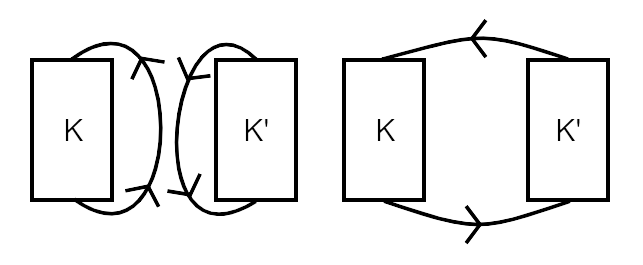
\includegraphics[width=0.9\linewidth]{img/nussuma.png}
	\caption{Suma de dos nusos qualssevol.}\label{fig:nussuma}
\end{figure}

La Figura \ref{fig:knotable} és una taula que conté tots els nusos primers de fins a 9 creuaments. Cadascun rep un nom conformat per un parell de nombres; el primer de tots correspon al seu ordre i el segon és un subíndex històricament assignat a aquell nus en concret. Les primeres tabulacions que es coneixen van fer-se per Tait l'any 1860 mentre aquest estudiava l'àtom. Aquesta taula negligeix el fet que possiblement un mateix nus $K$ sigui diferent a $\overline{K}$, $rK$ o $\overline{rK}$. D'aquesta manera, cada nus de la taula correspon a un, dos o quatre nusos de $S^3$ mitjançant les operacions definides a \ref{def:nusemmirallat} i \ref{def:nusinvers}.

\begin{figure}
	\centering
	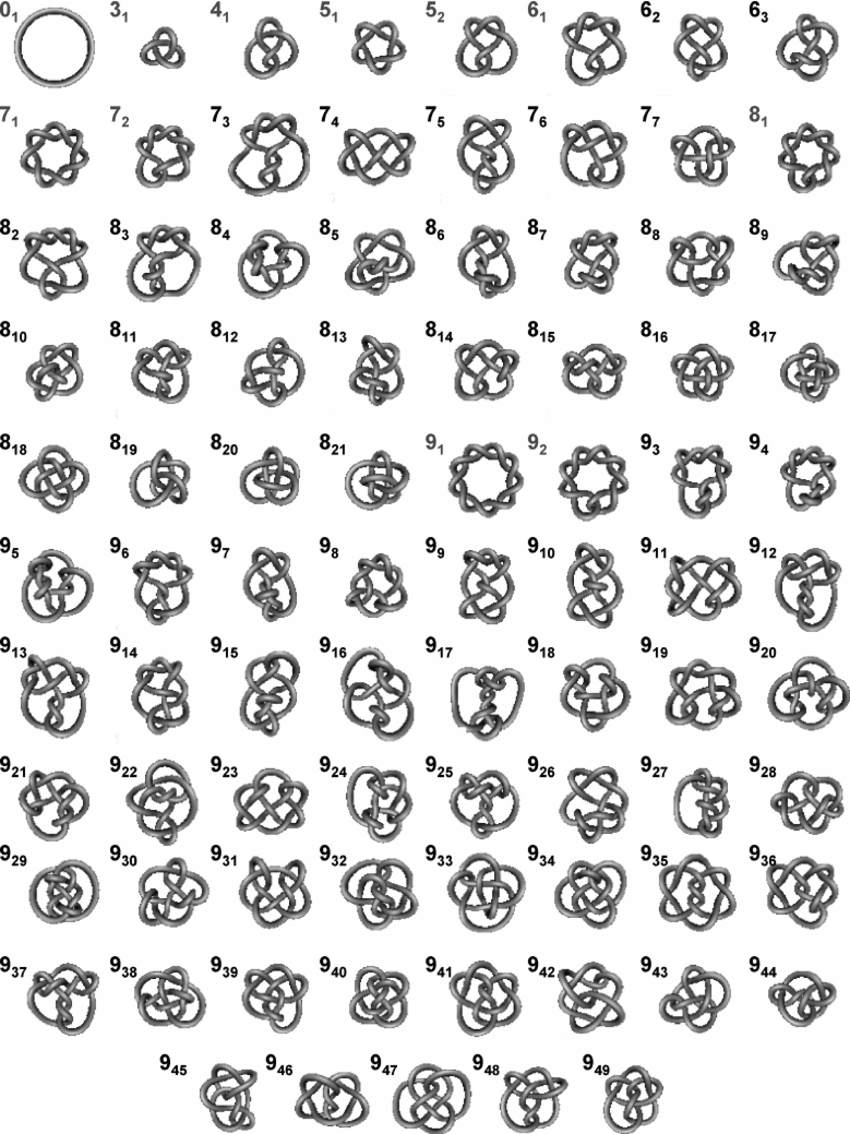
\includegraphics[width=0.9\linewidth]{img/knottable.png}
	\caption{Taula de nusos fins a ordre 9.}\label{fig:knotable}
\end{figure}

\begin{definition}\label{def:nusalternat}
	Diem que $K$ és un nus \underline{alternat} si a mesura que anem recorrent el nus, els creuaments alternen de sobrepassos a sotapassos.
\end{definition}

El nus $4_1$ n'és un exemple. De fet, cal anar fins a $8_{19}$ per trobar el primer nus no alternat i doncs això és una conseqüència del baix ordre dels nusos. Es pot veure que donat un ordre qualsevol, sempre existeix com a mínim un nus alternat. Ara bé, aquests disminueixen exponencialment a mesura que incrementem l'ordre del nus. Aquesta classe de nusos tenen bones propietats.